% !BIB TS-program = biber
\documentclass[12pt]{article}

\usepackage{listings}
\usepackage[left=25mm, top=30mm, bottom=20mm, right=25mm, headsep=10mm]{geometry}
\usepackage[utf8]{inputenc}
\usepackage[german]{babel}
\usepackage{fancyhdr}
\usepackage{graphicx}
\usepackage{color, colortbl}
\usepackage{tabularx}
\usepackage{helvet}
\usepackage[table,xcdraw]{xcolor}
\usepackage{enumitem}
\usepackage{parskip}
\usepackage{float}

\usepackage[sorting=none]{biblatex}

\addbibresource{references.bib}

\setlength{\parindent}{0pt}

\newcommand{\subsubsubsection}[1]{\paragraph{#1}\mbox{}\\}
\setcounter{secnumdepth}{4}
\setcounter{tocdepth}{4}

% ============== START Header and Footer ============== %
% http://tug.ctan.org/info/german/fancyhdr/fancyfolien+bsp.pdf
\pagestyle{fancy}
\renewcommand{\headrulewidth}{.5pt}
\fancyhead[OL,EL]{\fontsize{9}{12} \selectfont Cloud Computing}
\fancyhead[OR,ER]{\fontsize{9}{12} \selectfont Kubernetes}

\renewcommand{\footrulewidth}{.5pt}
\fancyfoot[OL,EL]{\fontsize{9}{12} \selectfont Berner Fachhochschule}
\fancyfoot[OC,EC]{\fontsize{9}{12} \selectfont \thepage}
\fancyfoot[OR,ER]{\fontsize{9}{12} \selectfont Lars Peyer, Adrian Berger}
% ============== END Header and Footer ============== %

\makeatletter
\setlength{\@fptop}{0pt}
\makeatother

\begin{document}
	
	\begin{titlepage}
	
	\begin{center}
		
\includegraphics[width=150mm]{media/titleimage.jpg}\\[10mm]	
		\line(1,0){450}\\[7mm]
		\huge{Cloud Computing \protect\\[10mm] Kubernetes}\\[2mm]
		\line(1,0){450}\\[2cm]
		\large{Peyer Lars}\\[3mm]
		\large{Berger Adrian}\\[15mm]
		\large{Version 0.1}\\[5mm]
		\today\\[20mm]
		
	\end{center}
\end{titlepage}
\newpage
	\renewcommand{\contentsname}{\vspace{-1.5cm}}
\tableofcontents
\newpage
	\section{Einleitung}
Dieses Dokument beinhaltet eine Übersicht zur Container-Orchestrierungsplattform Kubernetes.

Damit diese Thematik erläutert werden kann, wird ein grundsätzliches Verständnis von Container Technologien (hauptsächlich Docker) vorausgesetzt.

Eine kurze Übersicht über Docker kann unter dem folgenden Link gefunden werden:  
 
https://www.redhat.com/en/topics/containers/what-is-docker
\clearpage
	\section{Übersicht}
\subsection{Was ist Kubernetes?}
\subsection{Wieso Kubernetes}
\subsection{Alternativen}
\clearpage
	\section{Architektur}
\begin{center}
	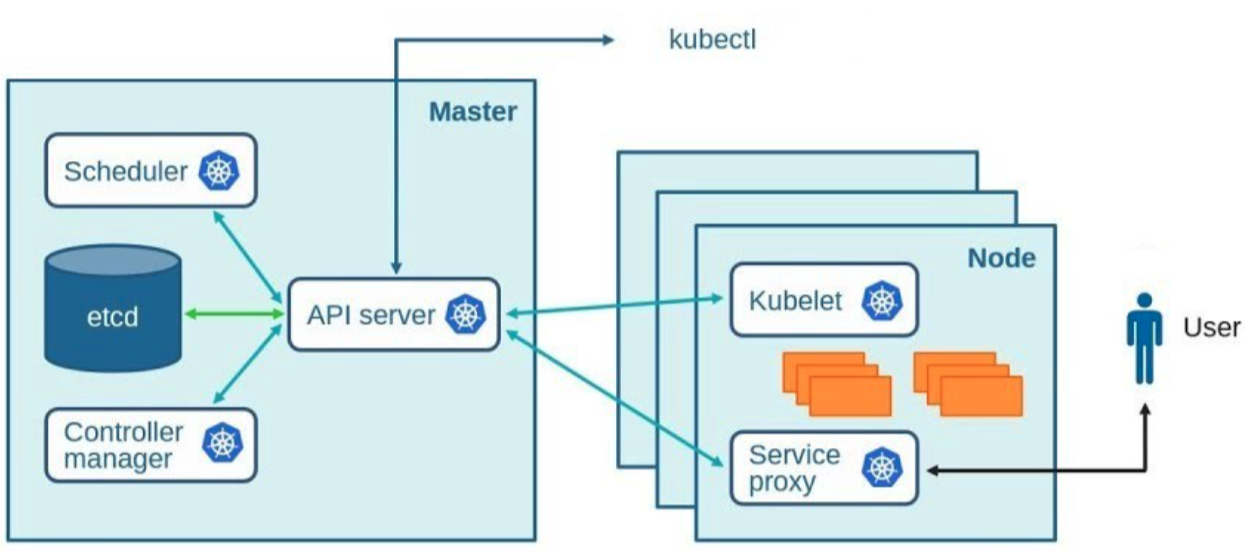
\includegraphics[height=50mm]{media/architektur.png}
\end{center}
\subsection{Master-Nodes}
Kubernetes funktioniert nach dem Master-Worker Prinzip.
Der Master Node ist dabei der Hauptknotenpunkt von Kubernetes. Er kontrolliert und koordiniert alle Aktionen, die im Cluster erfolgen. Fällt der Master-Node in einem Cluster aus, so wird dieser disfunktional. Die Node Server warten auf Befehle vom Master und führen diese anschliessend aus. Folgende Hauptkomponenten sind Bestandteil eines Kubernetes Master-Nodes und werden auch Control-Plane genannt.  \cite{kubernetes}
\subsubsection{API Server}
Der API-Server ist die Drehscheibe des Kubernetes-Cluster und ist zuständig für die Entgegennahme und Verteilung von Aufträgen wie z.B. Deployments oder Konfigurationen. Alle Komponenten des Clusters (Master- und Worker-Node) sind an den API Server angeschlossen und tauschen so untereinander Status-Informationen übern Den Cluster-Zustand aus. \cite{kubernetes}
\subsubsection{Scheduler}
Der Scheduler kennt alle verfügbaren Ressourcen im Cluster und der Zustand aller verbundenen Worker-Nodes. Wird über den API Server ein neues Deployment in Auftrag gegeben, sucht sich der Scheduler einen passenden Worker-Node raus, welcher über die benötigten Ressourcen (CPU, RAM, DISK) verfügt. Er meldet die passenden Worker-Nodes dem API-Server, welcher dann das Deployment auf den ausgewählten Nodes ausführt. \cite{kubernetes}
\subsubsection{Controller manager}
Der Controller manager besteht eigentlich aus vier Subkomponenten, welche zu einem Controller zusammengeführt werden. 

Der \textbf{Node-Controller} überwacht den Zustand aller Worker-Nodes im Cluster. Fällt eine Node aus, schaut der Controller ob die Node neu gestartet werden kann oder ob eine neue Node erstellt werden muss.

Der \textbf{Replication-Controller} ist zuständig dafür, dass alle Deployments gemäss Konfiguration repliziert werden. Sollte ein Worker-Node ausfallen, werden über den Replication-Controller neue Replikationen auf anderen Worker-Nodes gestartet.

Der \textbf{Endpoint-Controller} baut die Verbindung zwischen allen Pods und Services her. Services werden dazu verwendet, dass Pods untereinander kommunizieren können.

Die \textbf{Service Account und Token Controllers} sind zuständig um neue Standardkonten beim Erstellen von Namespaces (Gruppierungen von Pods) zu kreieren. Zudem verwalten sie die Zugriffstokens des API Severs damit nicht einfach jeder auf den Cluster zugreifen kann. \cite{kubernetes}
\subsubsection{Etcd}
Etcd ist ein externer hoch konsistenter Key-Value Store, welcher speziell auf Verteilte Systeme ausgelegt ist und die wichtigsten Daten des Kubernetes Cluster ablegt. Es werden sämtliche Konfigurationen und Zustände des Systems im Etcd Store abgelegt. Dadurch empfiehlt es sich diesen Store zu replizieren, denn bei einem Ausfall sind alle Cluster Daten verloren und der Cluster somit unbrauchbar. \cite{kubernetes}

\subsection{Worker-Nodes}
Worker-Nodes sind Arbeitstiere und stellen dem Cluster die Ressourcen zur Verfügung um Applikationen bereit zu stellen. Dabei handelt es sich meist um virtuelle Maschinen oder kleine physische Maschinen, welche zu einem grossen Netzwerk zusammen geführt werden. Ein Master-Node kann maximal bis zu 5000 Worker-Nodes unter sich verwalten. \cite{kubernetes}
\subsubsection{Kublet}
Auf jedem der Worker-Nodes läuft der Kublet-Dienst. Dieser ist für die Kommunikation im Cluster zuständig und verbindet sich mit dem API Server damit Statusinformationen und Konfiguration ausgetauscht werden können. Dieser Dienst ist das Herzstück des Worker-Nodes und kommuniziert mit der Container Runtime (meistens Docker), welche auf dem Node installiert ist, damit Pods und Containers erstellt werden können. \cite{kubernetes}
\subsubsection{Pod}
Ein Pod ist die kleinste verwaltbare Einheit in einem Kubernetes Cluster un beinhaltet einen oder mehrere Containers. Alle Container im Pod teilen sich die definierten Konfigurationen und die geteilten Speicher- und Netzwerk-Ressourcen. Es empfiehlt sich nur stark verbundene Container, welche sich gegenseitig ergänzen, in einem Pod zusammen zu fassen. In den meisten Fällen befindet sich lediglich ein Container in einem Pod. \cite{kubernetes}
\subsubsection{Container}
Container werden auf Basis von einem Container-Abbild gestartet und beinhalten alles was die Applikation benötigt um lauffähig zu sein. Der Container verwendet zum Betrieb des Abbilds die Ressource, welche ihm durch die Container Runtime zur verfügung gestellt werden. Am weitesten verbreiten sind Docker Container, welche aus einem Docker-Image gestartet werden. In einem YAML-File (Dockerfile) wird die Applikation konfiguriert und mittels Docker zu einem Image gebaut.  \cite{kubernetes}
\subsubsection{Service proxy}
Damit Pods im Cluster miteinander kommunizieren können, werden Services eingesetzt. Dabei wird definiert bei welchem Pod welche Ports geöffnet sind und über welche lokale IP die Pods miteinander kommunizieren können.

Pods können zur internen Kommunikation anstelle der IP Adresse auch einfach über den Service-Name angesprochen werden. Dies ist vor allem bei replizierten Applikationen interessant, da die Anfragen-Verteilung auf die verschiedenen Replikationen nicht manuell gemacht werden muss. 
Zudem dient der Service Proxy für den Benutzer der Zugangspunkt einer Applikation.  \cite{kubernetes}

\subsection{Schnittstellen}
\subsubsection{kubectl}
Kubectl ist eine Applikation, welche in der Kommandozeile läuft und zur Konfiguration von Kubernetes Clustern dient. Dies Applikation ist direkt mit dem API Server verbunden und bieten eine Vielzahl an Befehlen um den Cluster zu konfigurieren oder Applikationen zu deployen. 
Deployment werden mittels YAML-Files geschrieben und können als Datei direkt dem Kubectl zur Übertragung an den Cluster übergeben werden. \cite{kubernetes}
\subsubsection{Web UI}
Alternativ zum Kubectl kann auch das Web UI zur Konfiguration des Clusters verwendet werden. Im Web UI erhält man eine schöne visuelle Übersicht über den Cluster und sieht mittels Graphen die Auslastung der einzlnen Komponenten. Die Konfiguration mittels Kubectl scheint aber um einiges schneller zu gehen und darum ist das Web UI mehr eine schöne Ergänzung dazu. \cite{kubernetes}
\clearpage
	\section{Beispiels-Applikation in einem Kubernetes Cluster}
Für unser Beispiel haben wir eine simple Applikation gewählt, die aus den folgenden Containern besteht:

Vue.js Frontend Container
Django Backend Container
Postgres Datenbank Container

Diese Aplliaktion soll nun bei Hetzner in einem Kubernetes Cluster betrieben werden.
\clearpage
	\printbibliography
	
\end{document}
